\section{Theoretical Foundations \& Runtime Necessity Model}

\subsection{Decision-Preserving Sufficiency (ST-015)}
A representation $R_t \in \mathcal{R}$ is \emph{decision-sufficient} with respect to optimal policy $\pi^*$ if:
\[
\pi^*(R_t) = \pi^*(S_t) \quad \forall S_t \in \mathcal{S}
\]

\subsection{Runtime Necessity Formalization (ST-016)}
We formalize a TAKT Governed Runtime as a tuple $M = (\mathcal{C}, \pi_M)$, where the capability set satisfies:
\[
\mathcal{C} \;\subseteq\; \{C_{\text{contract}},\; C_{\text{uncertainty}},\; C_{\text{temporal}}\}
\]

\begin{figure}[htbp]
\centering
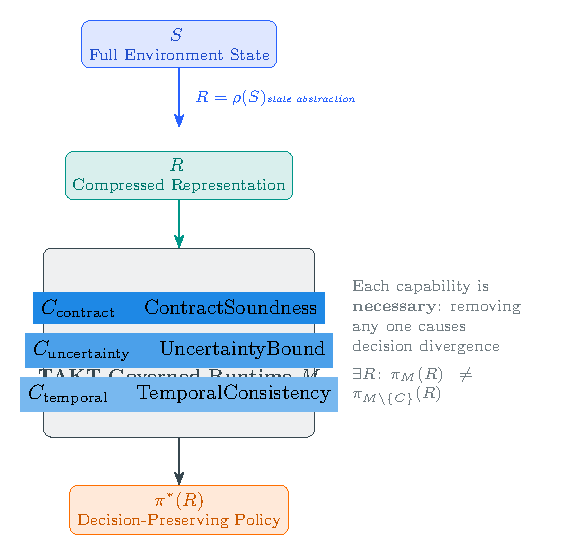
\includegraphics[width=0.85\linewidth]{figures/architecture.pdf}
\caption{Conceptual architecture: TAKT Governed Runtime $M$ enforces decision
preservation $\pi^*(R)$ under state abstraction $\rho(S)$.}
\label{fig:architecture}
\end{figure}

\textbf{Definition (Capability Necessity):} A capability $C \in \mathcal{C}$ is
\emph{locally necessary} for runtime $M$ if removing $C$ alters policy decisions
on at least one representation:
\[
\exists\, R \in \mathcal{R}:\; \pi_M(R) \;\neq\; \pi_{M \setminus \{C\}}(R)
\]

\textbf{Example 1 (Temporal Prefix Necessity):} Consider a runtime where
$C_{\text{temporal}}$ is ablated. Two trajectories $\tau_1 = (r_0, r_1, r_2)$
and $\tau_2 = (r'_0, r'_1, r_2)$ share an identical terminal state $r_2$.
If $\tau_1$ is safe and $\tau_2$ is unsafe, a runtime inspecting only $r_2$
assigns identical actions — causing decision divergence $\pi_M(\tau_1) \neq \pi^*(\tau_1)$.
